\documentclass[11pt, spanish, a4paper]{article}
\usepackage[spanish]{babel}
\usepackage[top=0.5in]{geometry}
\selectlanguage{spanish}
\usepackage[utf8]{inputenc}
\usepackage{hyperref}
\usepackage{mathtools}
\usepackage{graphicx}
\graphicspath{ {images/} }
\usepackage{amsmath}


\author{Marco Moresi}
\begin{document}
\title{Laboratorio Número 1 Aprendizaje Automático en Visión por Computadoras}
\maketitle

\tableofcontents

\section{Introducción}
En el presente informe se muestran los resultados del trabajo propuesto por la cátedra, el objetivo propuesto es familiarizarse con el \textbf{pipeline} de trabajo que habitualmente se utiliza en los proyectos de Aprendizaje Automático aplicado en Visión por Computadoras.
A continuación se enumeran las consignas, luego para cada consigna se describe el trabajo realizado junto con los resultados y gráficos pertinentes.

\section{Consignas}

[0] Familiarizarse con el código y con el dataset.

\hyperref[ejercicio1]{[1]} Determinar el mejor valor para el parámetro C del clasificador (SVM lineal)
mediante 5-fold cross-validation en el conjunto de entrenamiento (gráfica) de
uno de los folds. Una vez elegido el parámetro, reportar media y desviación
estándar del accuracy sobre el conjunto de test.

\hyperref[ejercicio2]{[2]} Evaluar accuracy vs. n\_clusters. Que pasa con los tiempos de cómputo de
BoVW?. Gráficas.

Si tengo descriptores locales L2-normalizados: cómo puedo optimizar la
asignación de los mismos a palabras del diccionario? (ayuda: expresar la
distancia euclídea entre dos vectores en términos de productos puntos entre los
mismo)

\hyperref[ejercicio3]{[3]} Transformaciones en descriptores / vectores BoVW: evaluar impacto de
transformación sqrt y norma L2.


\hyperref[ejercicio4]{[4]} Kernels no lineales: Intersección (BoVW: norm=1) y RBF, ajustando parámetros
mediante cross-validation en conjunto de validación.



\section{Ejercicios}
\subsection{Ejercicio 1}
\label{ejercicio1}
Como base se utilizó el archivo \href{https://drive.google.com/file/d/0B6mRi0ta2K1rRmRmRUlTblNzX0k/view?usp=sharing}{lab.py}, para realizar \textbf{5-fold cross-validation}, se dividió el set de entrenamiento en 5 partes iguales, se tomaron las 4 primeras partes como \textbf{train\_set} y última partición como \textbf{validation\_set} se entrenaba y validaba el clasificador lineal (SVM Lineal) para cada valor C y se guardaba la medida de \textbf{accuracy} obtenida para cada valor de C en su respectiva lista. Luego concatenaba la partición correspondiente al \textbf{validation\_set} al inicio del \textbf{train\_set} y volvia a tomar las 5 particiones, del mismo modo que se menciona mas arriba, de esta forma tanto el \textbf{validation\_set} como el \textbf{train\_set} variaban en cada iteración.

Para llevar a cabo esta tarea se considero como primera instancia la siguiente lista de posibles valores:

$$list\_C = [10^{-3}, 10^{-2}, 10^{-1}, 10^0, 10^1, 10^2, 10^3]$$

Luego de la ejecución arrojó los siguientes valores:

\[
10^{-3}=
  \begin{bmatrix}
	0.37 & 0.36 & 0.366 & 0.416 & 0.386
  \end{bmatrix}
\]

\[
10^{-2}=
  \begin{bmatrix}
	0.453 & 0.46 & 0.463 & 0.506 & 0.49
  \end{bmatrix}
\]

\[
10^{-1}=
  \begin{bmatrix}
	0.546 & 0.596 & 0.563 & 0.616 & 0.596
  \end{bmatrix}
\]

\[
10^{0}=
  \begin{bmatrix}
	0.603 & 0.636 & 0.623 & 0.64 & 0.64
  \end{bmatrix}
\]

\[
10^{1}=
  \begin{bmatrix}
	0.613 & 0.646 & 0.61 & 0.633 & 0.633
  \end{bmatrix}
\]

\[
10^{2}=
  \begin{bmatrix}
	0.596 & 0.573 & 0.573 & 0.596 & 0.603
  \end{bmatrix}
\]

\[
10^{3}=
  \begin{bmatrix}
	0.503 & 0.493 & 0.526 & 0.553 & 0.52
  \end{bmatrix}
\]



Luego de tomar la media a cada lista obtenemos el siguiente resultado:
$$list\_median = \begin{bmatrix} 0.37 & 0.463 & 0.596 & 0.636 & 0.633 & 0.596 & 0.520 \end{bmatrix}$$
\\
\textit{Anotacion: Los índices de list\_median coinciden con los de list\_C \\
e.g $C=10^{-3}$  $media = 0.37 $} \\


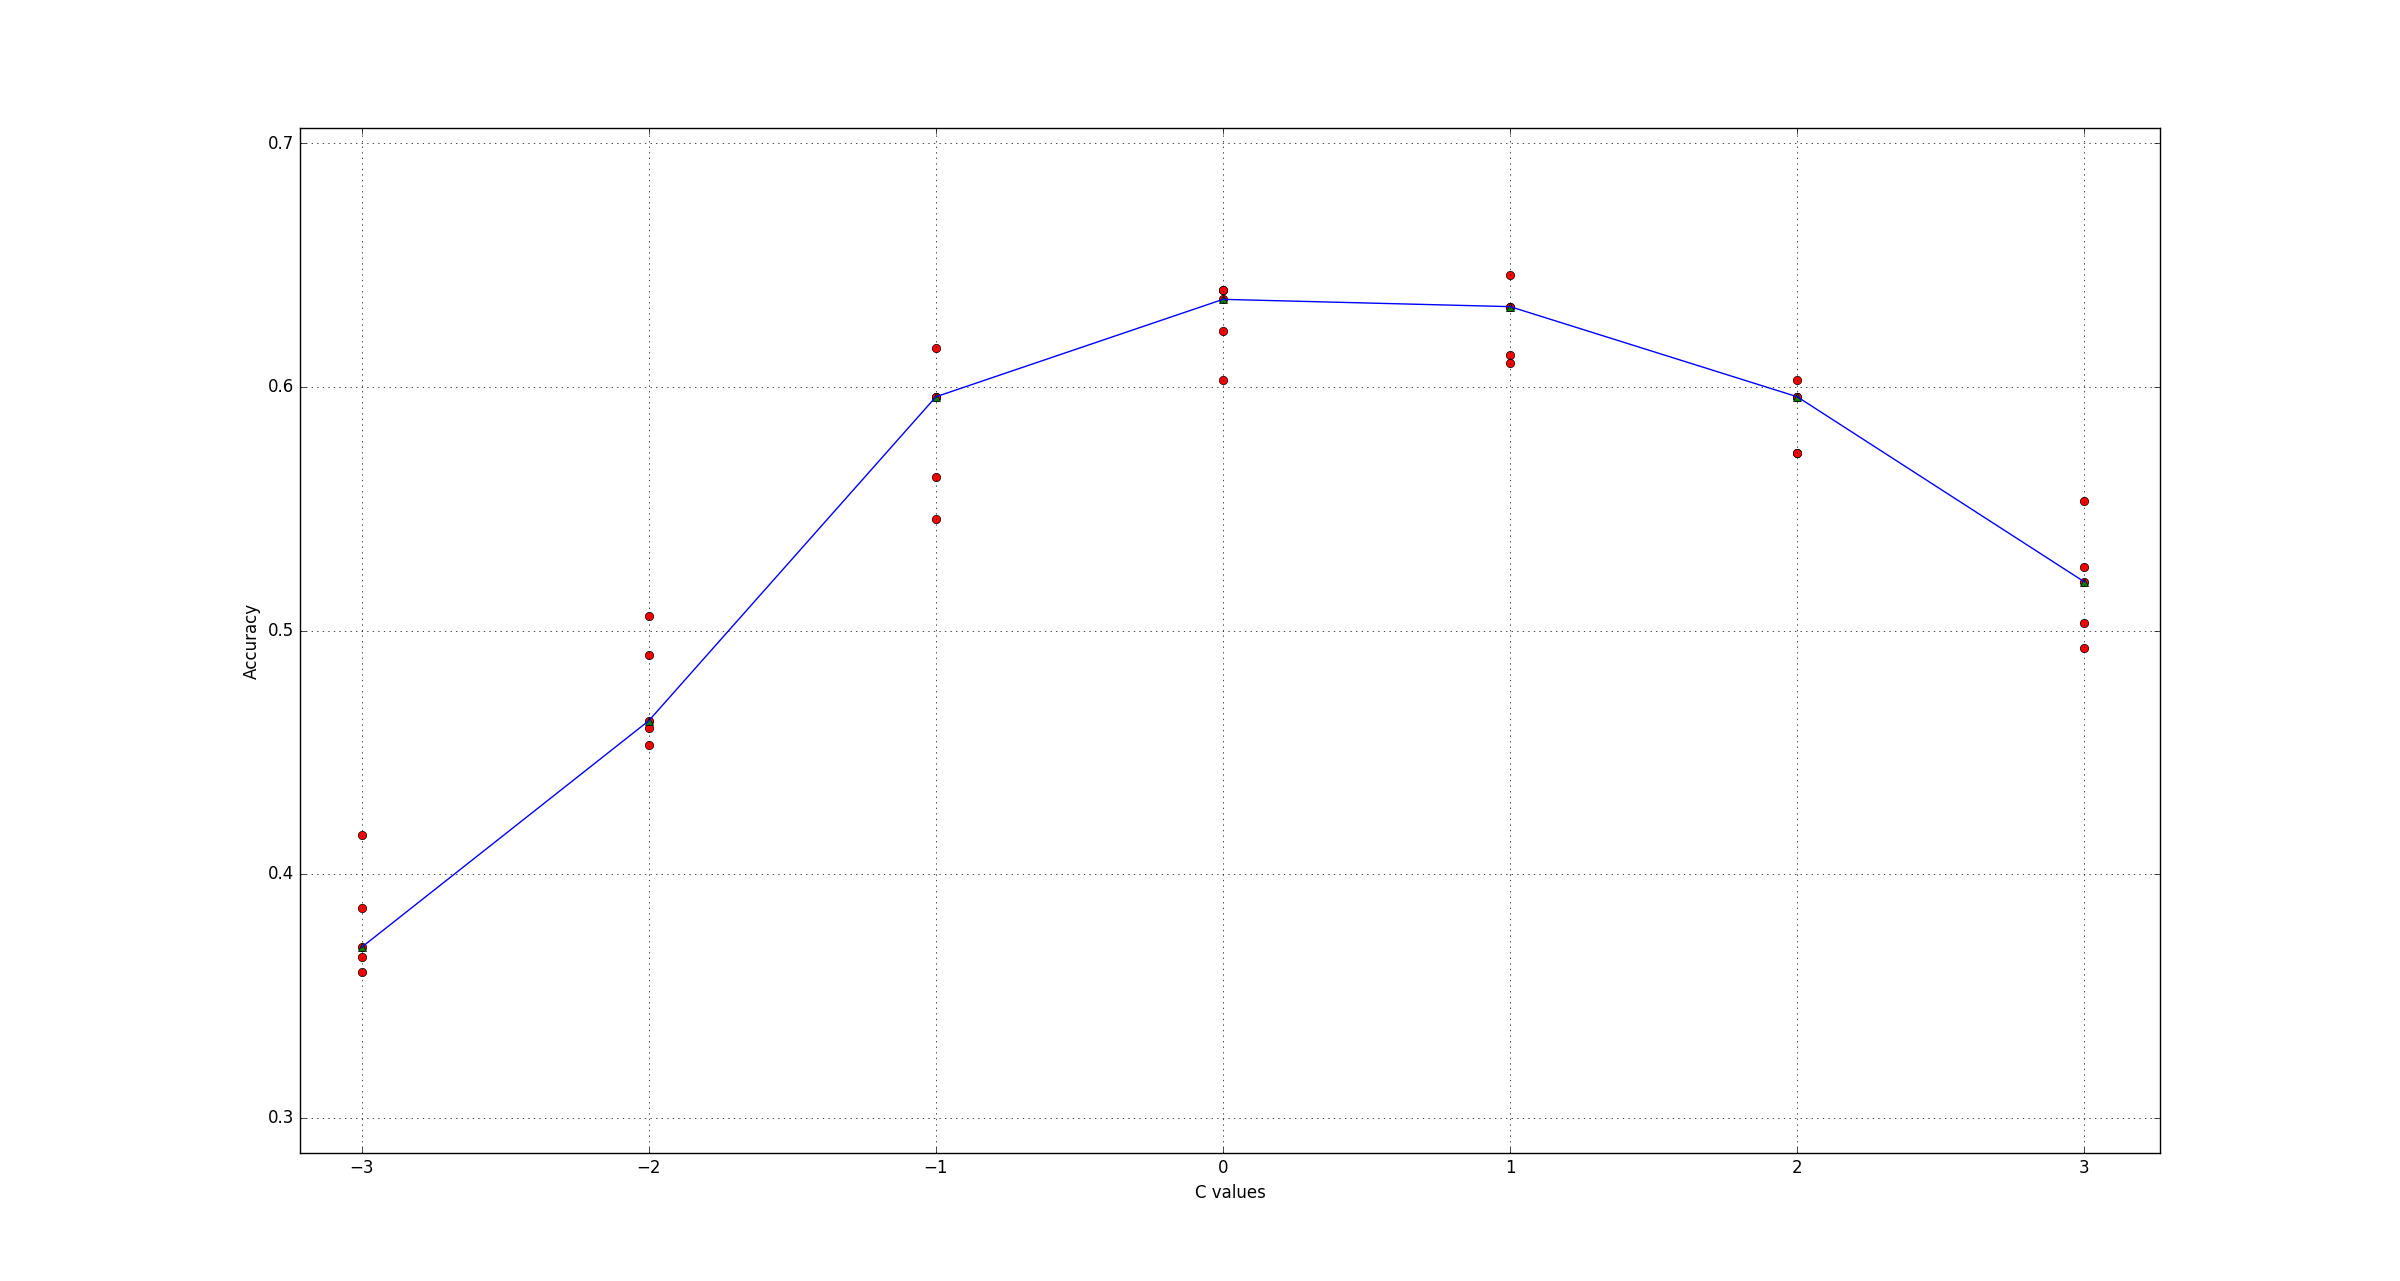
\includegraphics[scale=0.5, width=\textwidth]{figure_1.png}


En la lista de medias, podemos ver que obtenemos mayores medias usando el parámetro C entre $[10^0, 10^1, 10^2]$\\

Por lo tanto, refiné el parámetro entre esos valores.
Para ello volví a realizar \textbf{5-fold cross-validation} pero esta vez con:

\textit{Anotación: Para no aumentar mucho la extensión del informe sólo muestro las medias obtenidas para cada valor de C, en estos pasos intermedios. Acá podrá encontrar los \href{https://docs.google.com/document/d/1D158FDx7AdrAAm8I0YpSBx6bWm-kD-P2EK3xNqMiJ7M/edit}{valores completos}.}

$$list\_C = [1, 3, 5, 7, 9, 10]$$

$$list\_median = \begin{matrix} [0.646 & 0.633 & 0.636 & 0.636 & 0.626 & 0.626] \end{matrix}$$

Ahora refino entre $0.1$ y $2$

$$list\_C = [0.1, 1, 2]$$
$$list\_median = \begin{matrix} [0.573 & 0.653 & 0.646]\end{matrix}$$

Refino entre 0.5 y 2
$$list\_C = [0.5, 1, 1.5, 2]$$
$$list\_median = \begin{matrix}[0.650 & 0.660 & 0.670 & 0.663]\end{matrix}$$


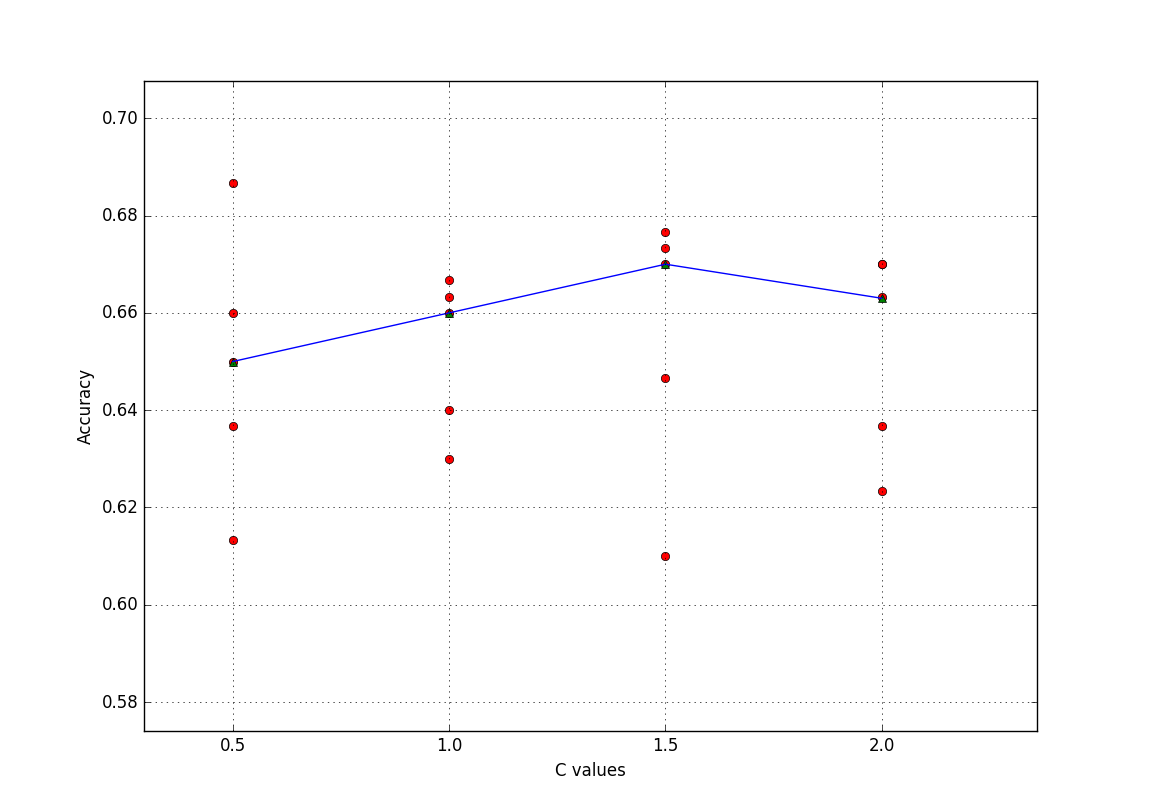
\includegraphics[scale=0.5, width=\textwidth]{figure_2.png}


Como obtuve la media mas grande en 1.5, ese será a partir de ahora mi parámetro C, para el clasificador lineal. \textbf{C=1.5}

Ahora voy a medir la media y la varianza que obtengo con el parámetro C escogido.
Para ello voy a ejecutar el pipeline 200 veces, variando el train\_set y el test\_set, tomando la medida de accuracy para cada corrida.

\textbf{Desviación standard = 0.0067  accuracy = 0.6538}



\subsection{Ejercicio 2}
\label{ejercicio2}
Accuracy Vs. N\_Clusters
Por defecto en \href{https://drive.google.com/file/d/0B6mRi0ta2K1rRmRmRUlTblNzX0k/view?usp=sharing}{lab.py} se utilizaban 100 clusters para ejecutar k-means. Lo que hice en este ejercicio fue probar distintos tamaños de clusters para el algoritmo K-means, medir cuanto tiempo demoraba en calcular los Bags of Visual Words y que accuracy obtenia el modelo con esa cantidad de clusters. Para ello definí una lista de posibles cantidad de clusters

$$clusters\_size = [1,5,10,25,50,75,100,110,125,140,150,175,200,250,300,325]$$

Luego para medir el tiempo de demora en computar los BOVW utilice la libreria de python llamada \href{https://docs.python.org/3.5/library/time.html}{time}. Entonces antes de computar los BOVW tomo el tiempo con time.time() y cuando termina de computarlos tomo nuevamente el tiempo y la resta de ellos, me da una aproximación al tiempo que demora en calcularlos. Despues de calcularlos, tomarle el tiempo elimino los BoVW y comienzo de nuevo.

Los resultados obtenidos fueron los siguientes:

\begin{center}
    \begin{tabular}{ | c | c | c |}
    \hline
    \textbf{N\_Clusters} & \textbf{Accuracy} & \textbf{Elapsed Time (Seg)}\\ \hline
    1 & 0.0472 & 4.4957    \\ \hline
    5 & 0.4177 & 6.3762 \\ \hline
    10 & 0.4606 & 8.1321 \\ \hline
    25 & 0.5504 & 13.7002 \\ \hline
    50 & 0.6100 & 22.8868 \\ \hline
    75 & 0.6428 & 30.9782 \\ \hline
    100 & 0.6566 & 40.1747 \\ \hline
    110 & 0.6753 & 42.3768 \\ \hline
    125 & 0.6646 & 48.1458 \\ \hline
    140 & 0.659 & 54.9081 \\ \hline
    150 & 0.683 & 57.8346 \\ \hline
    175 & 0.682 & 66.0863 \\ \hline
    200 & 0.683 & 75.4143 \\ \hline
    250 & 0.679 & 92.0769 \\ \hline
    300 & 0.663 & 109.572 \\ \hline
    325 & 0.661 & 118.4008 \\ \hline
    \end{tabular}
\end{center}


En el primer gráfico podemos ver el nivel de Accuracy en función de la cantidad de clusters, se observa que en N\_Clusters = 150 y N\_Clusters = 200 se alcanza el valor máximo de accuracy = 0.683. Entre 150 y 200 clusters tenemos una meseta en la función y luego de esto decae la performance.\\

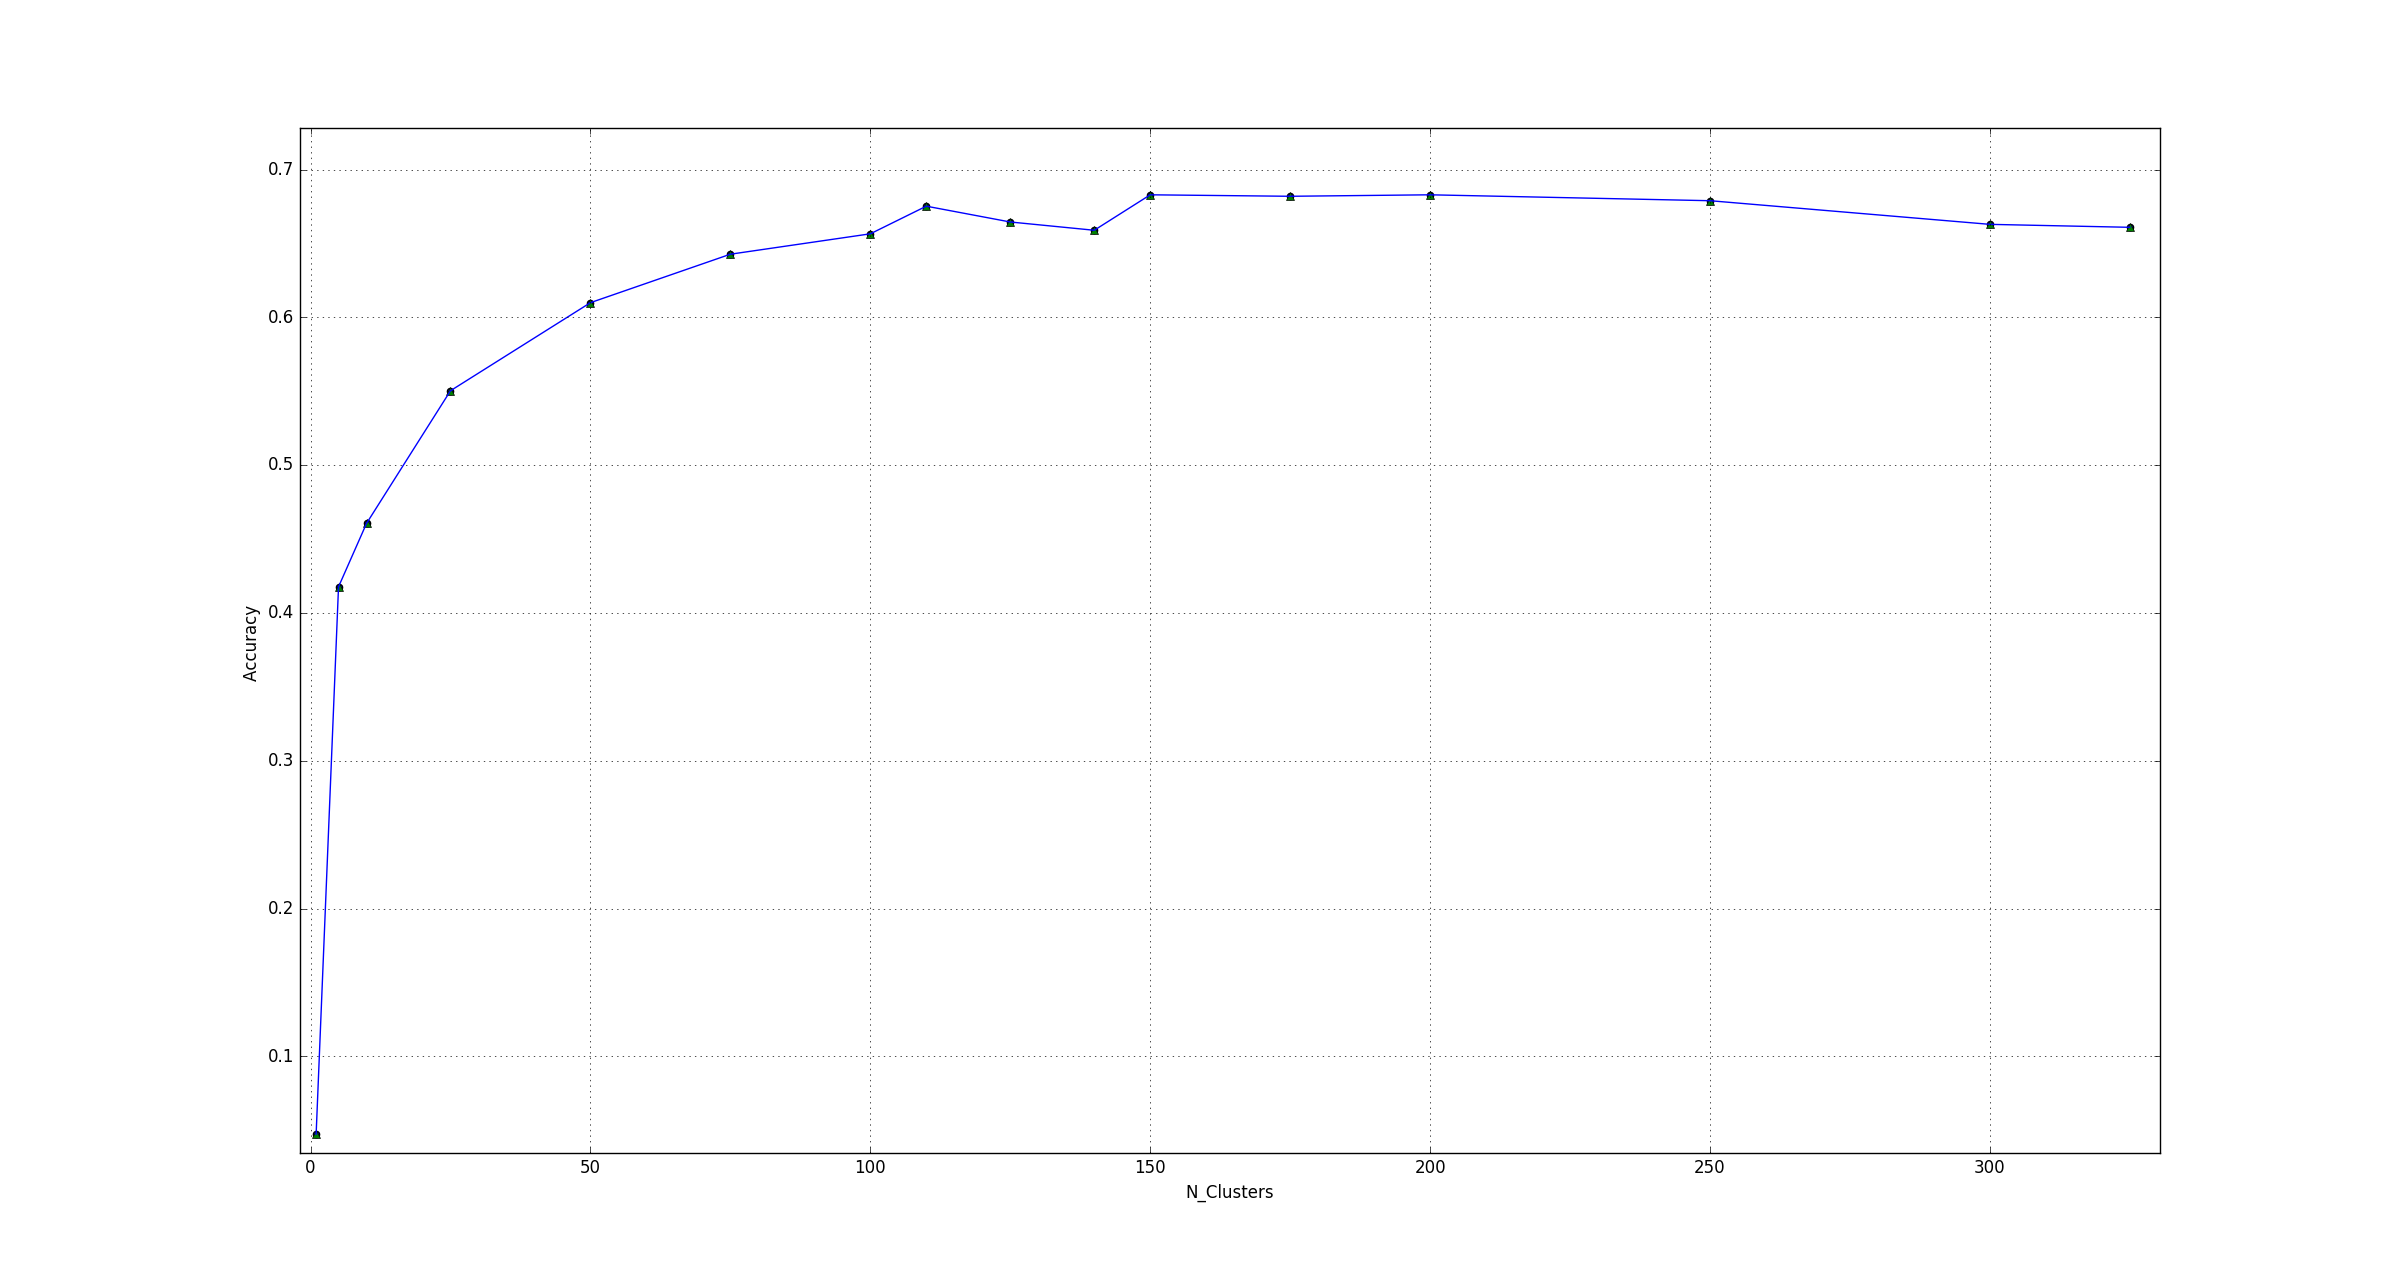
\includegraphics[scale=0.5, width=\textwidth]{figure_3.png}\\

Veamos ahora cuanto demora en calcular los BOVW, si nos centramos donde alcanza la mayor accuracy vemos que en N\_Clusters = 150 demora 57.8346 segundos aproximadamente mientras que en N\_Clusters = 200 demora 75.4143 aproximadamente.

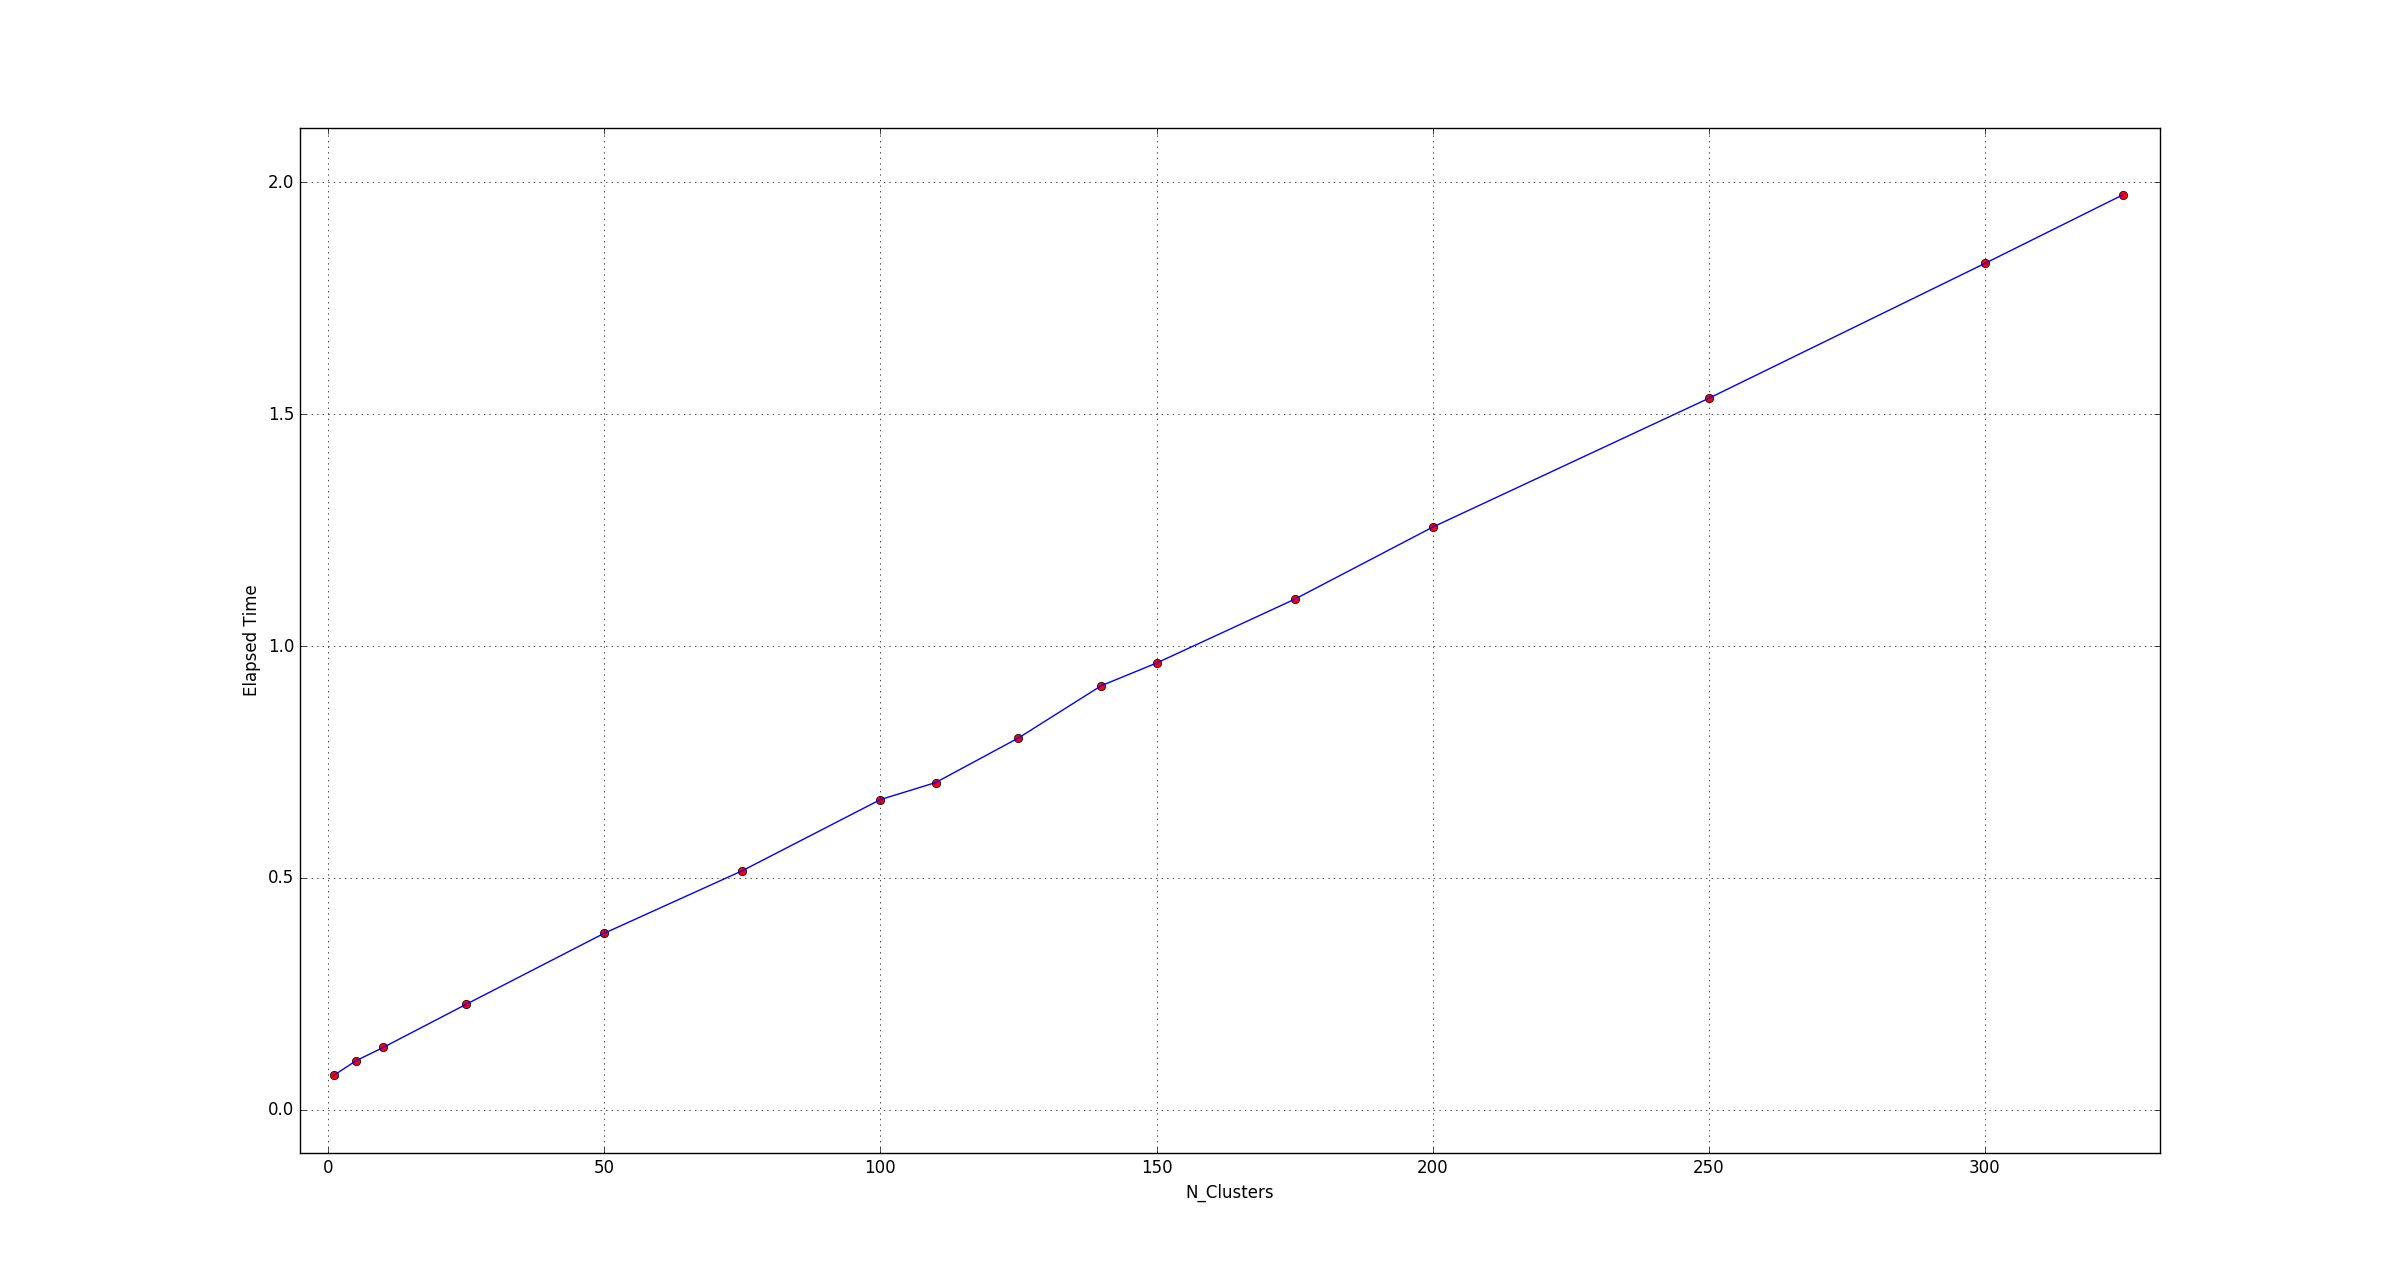
\includegraphics[scale=0.5, width=\textwidth]{figure_4.png}\\

Ahora si podemos ambas funciones en el mismo gráfico, podemos ver como a medida que mas clusters usamos mayor es el tiempo que demanda para computar los BOVW, pero no necesariamente obtenemos mayor accuracy. \\

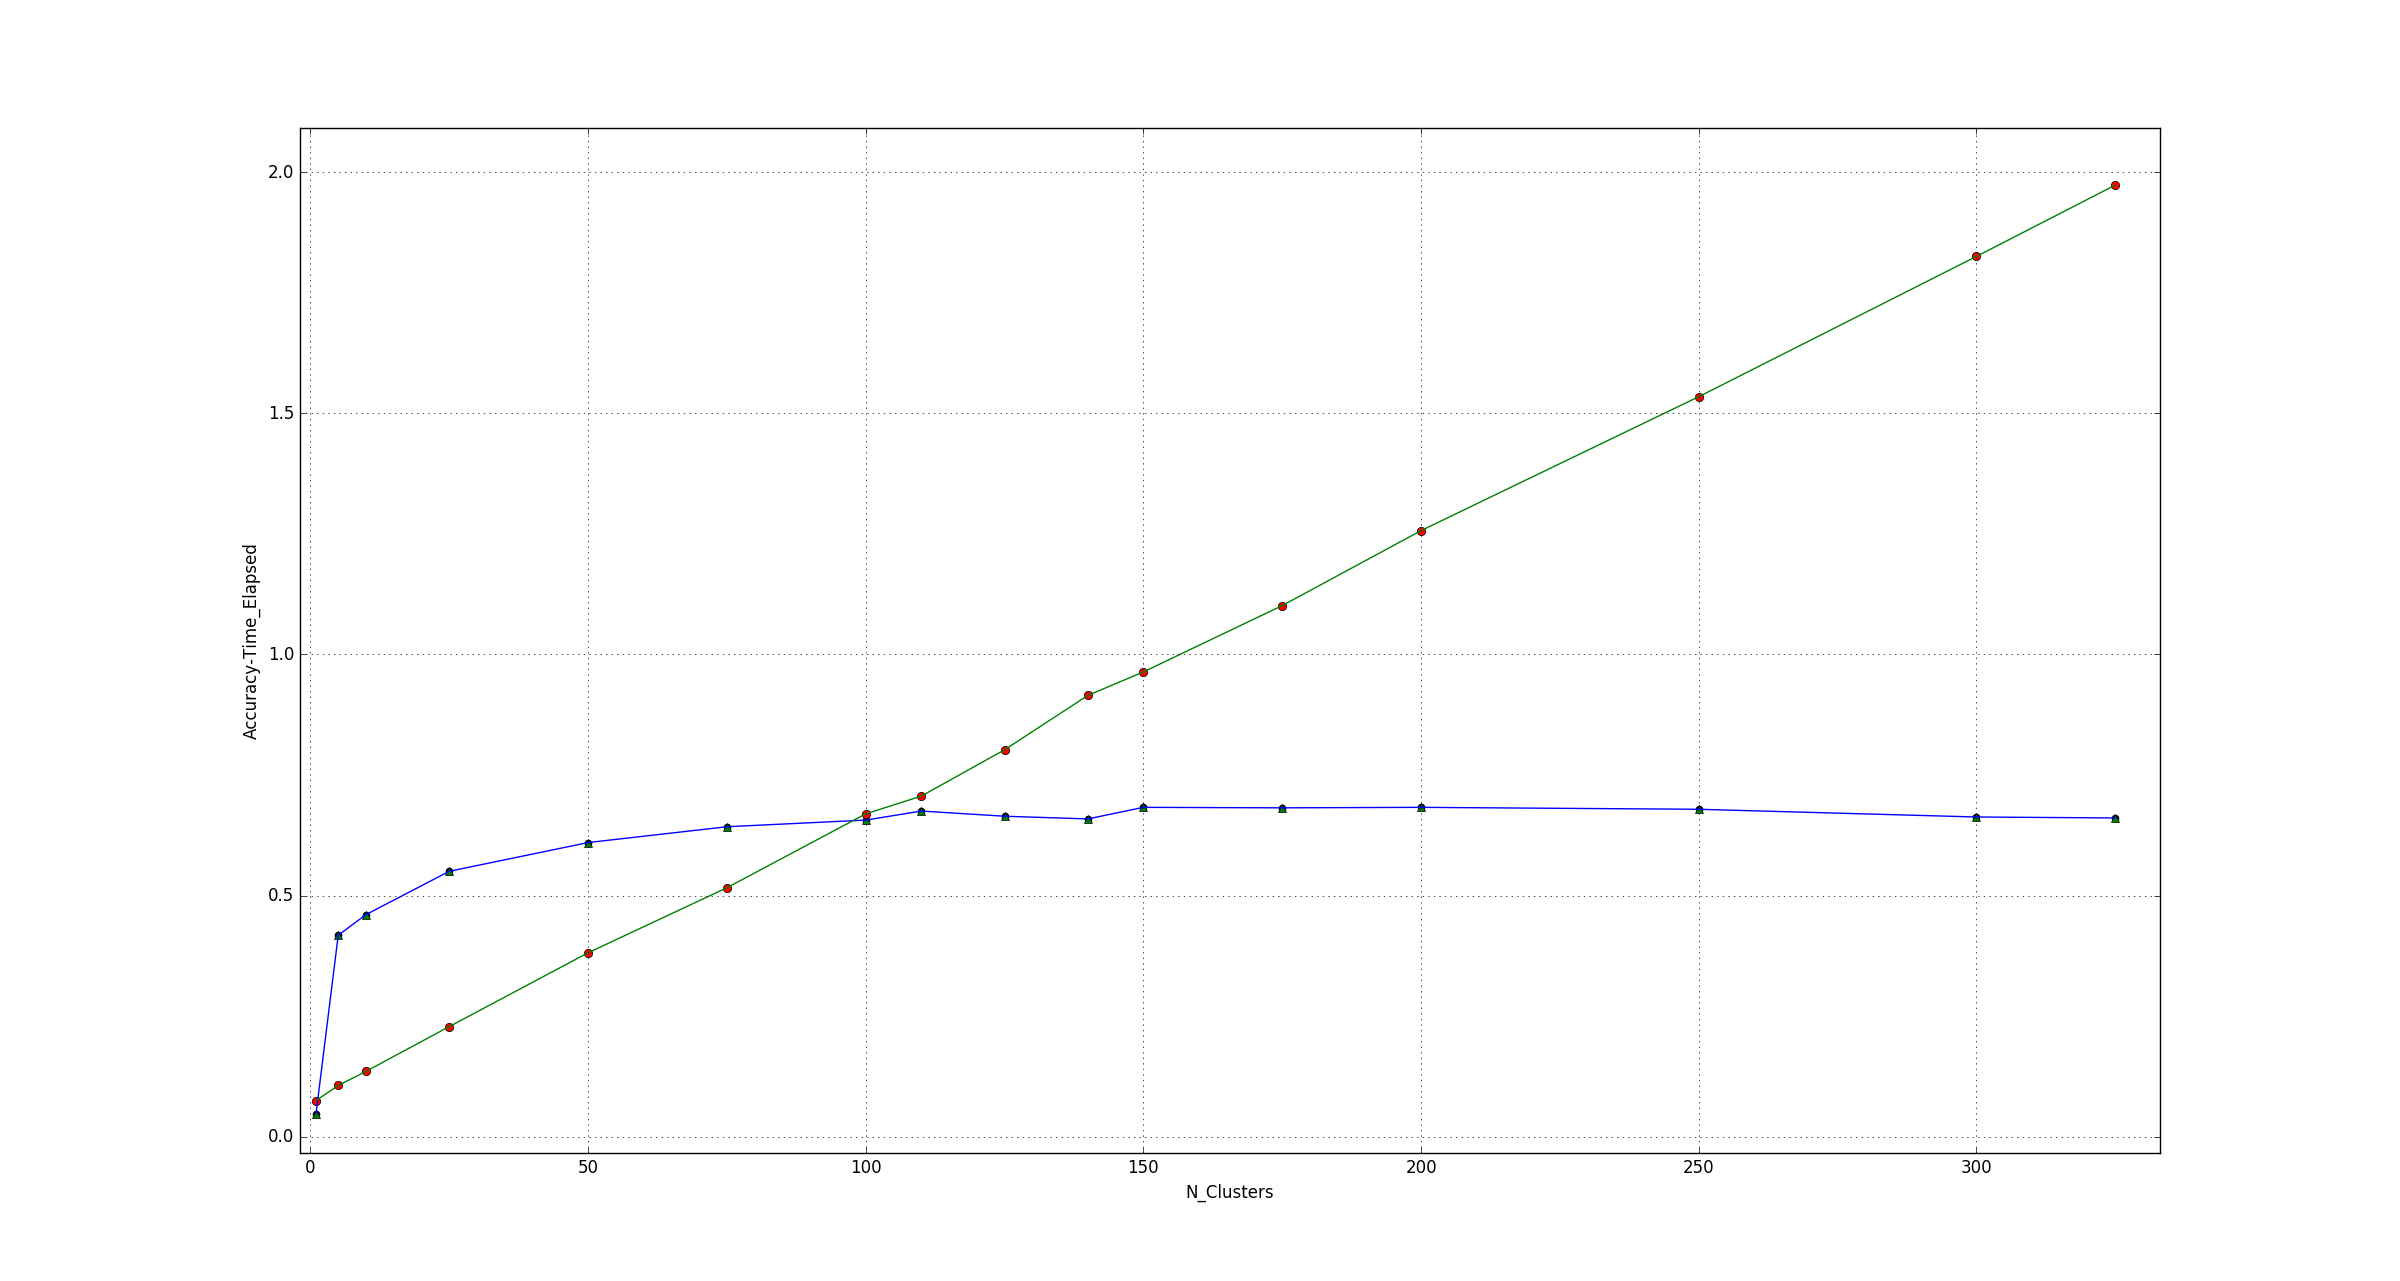
\includegraphics[scale=0.5, width=\textwidth]{figure_5.png}\\

\textit{Anotación: El tiempo está expresado en minutos para que sea más fácil la visualización y sea evidente lo que menciono mas abajo} \\
\\
Teniendo en cuenta el Trade Off entre tiempo de cálculo y accuracy la mejor elección en este caso es usar N\_Clusters = 150, que es el punto donde la función de la accuracy alcanza su máximo y esta lo más cerca posible de la función del tiempo.\\
De ahora en adelante considero \textbf{n\_clusters = 150}

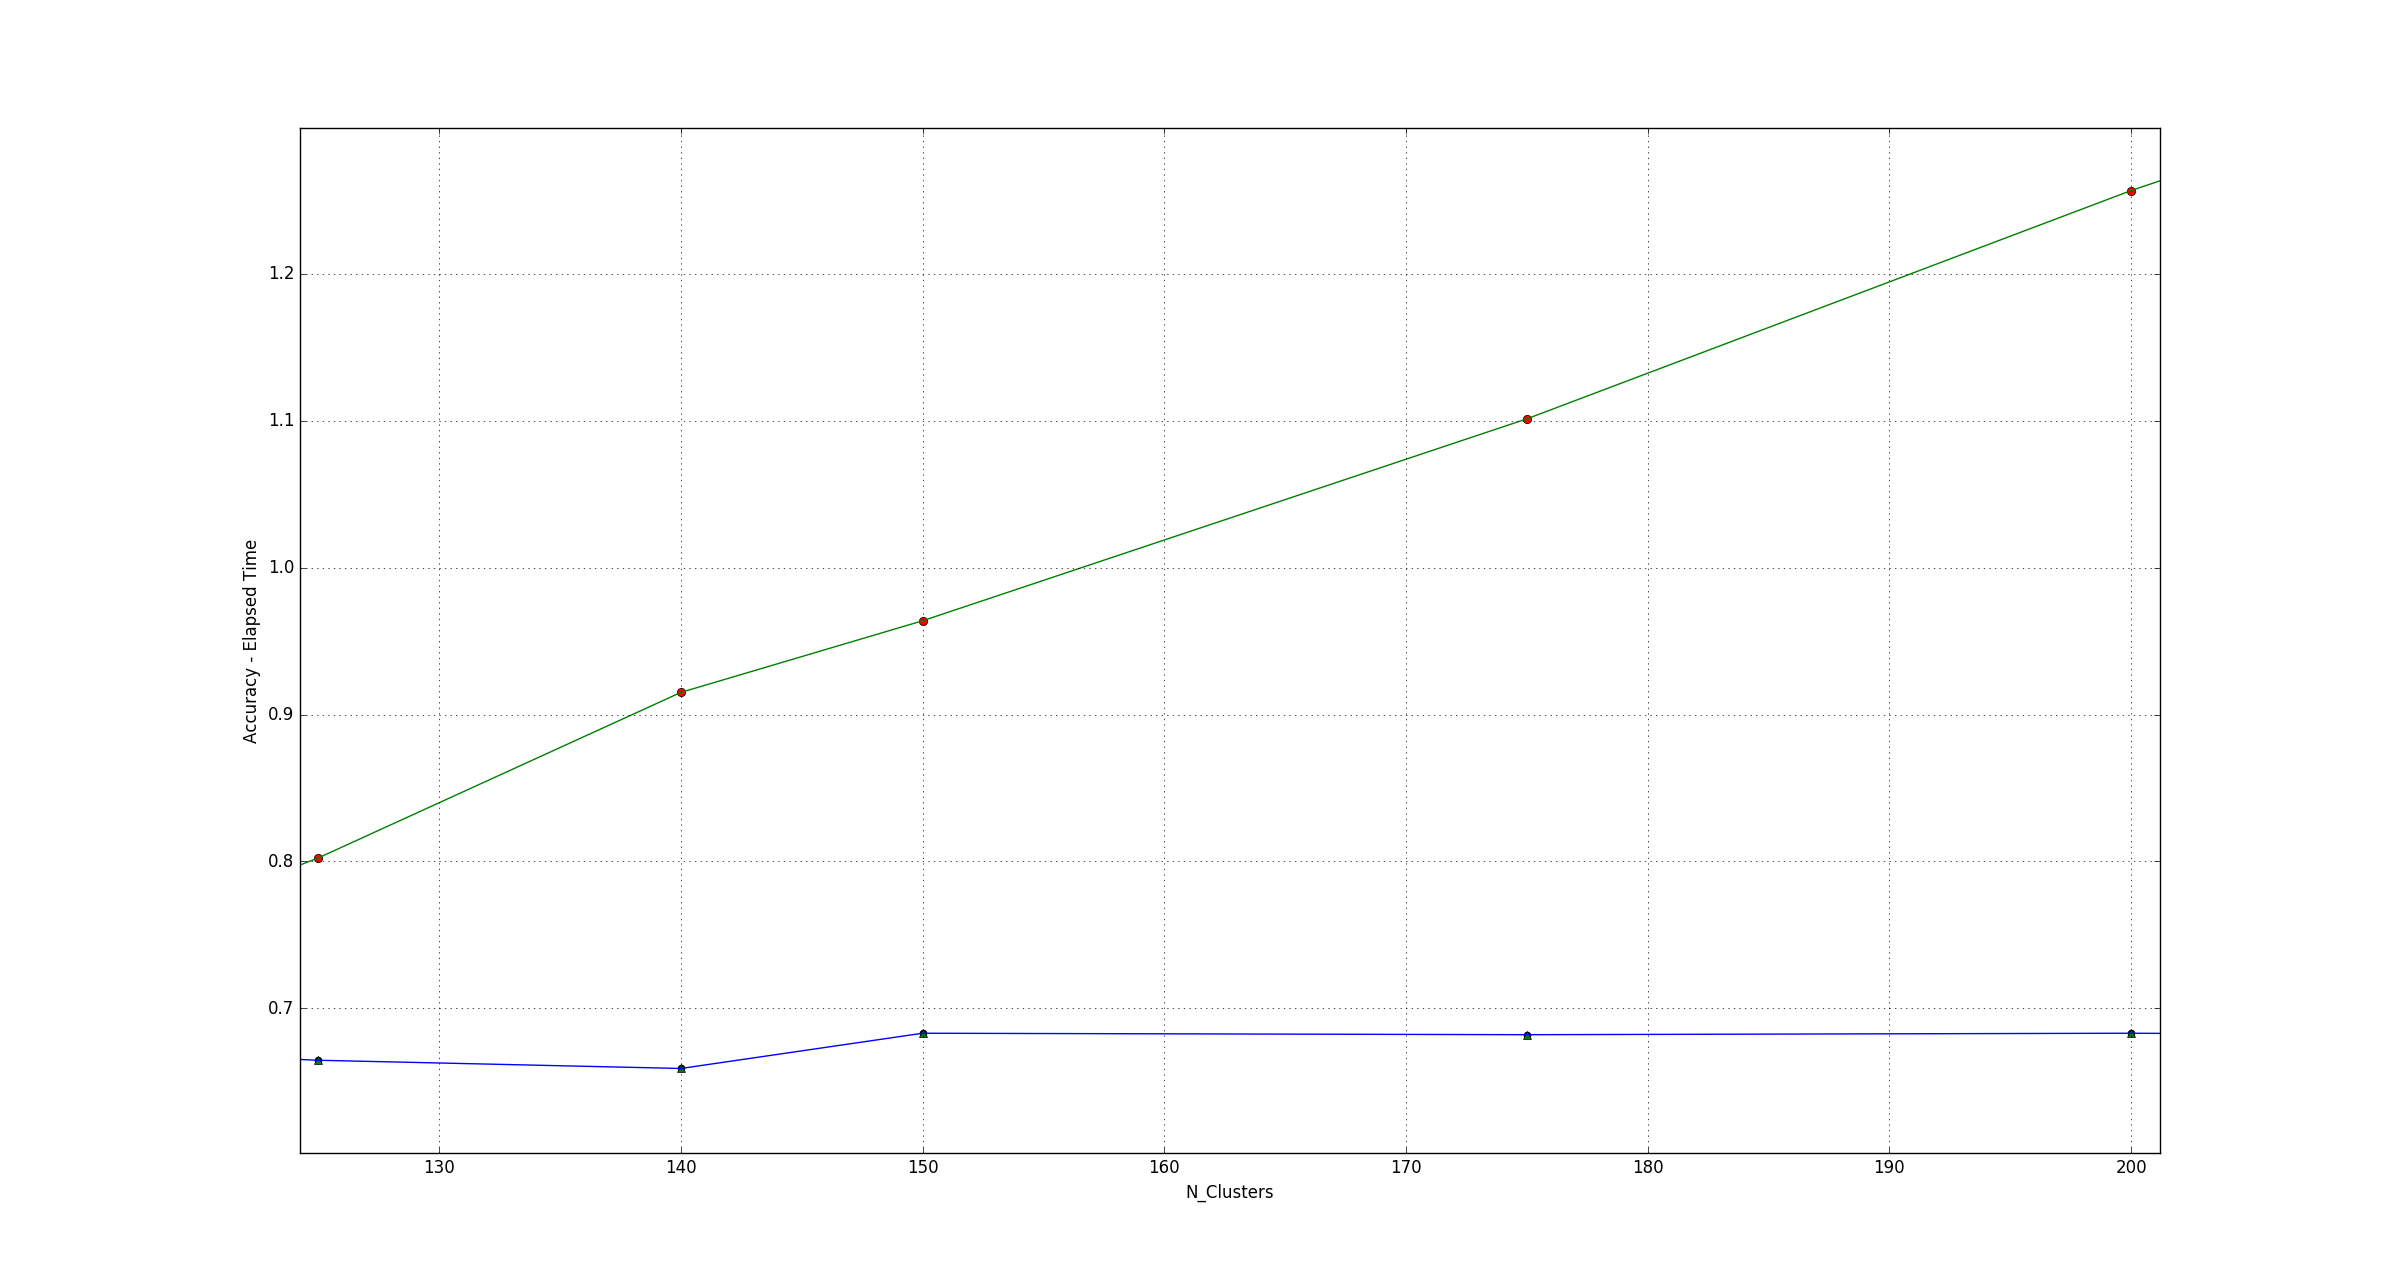
\includegraphics[scale=0.5, width=\textwidth]{figure_6.png}\\

\textbf{¿Cómo puedo optimizar la asignación de los mismos a palabras del diccionario?}


Para optimizar la asignación lo que podría hacer es computar la distancia Euclidea como producto punto de vectores, esto es computacionalmente más rapido ya que los microprocesadores traen instrucciones que resuelven los productos puntos en muy poco tiempo.
Vamos a escribir la distancia Euclidea entre dos vectores a y b como producto punto de ellos.

Primero defino (1): $||x||^2 = x^Tx = \displaystyle\sum_{i=1}^{n} (x_i x_i)$

Veamos ahora la distancia Euclidea (L2)
$$||a - b||_2^2 = \displaystyle\sum_{i=1}^{n} (a_i - b_i)^2 = (a-b)^T(a-b) = a^Ta-2a^Tb-b^Tb $$

Aplicamos (1), obtenemos
$$ = ||a||^2 -2a^Tb - ||b||^2 $$

Entonces
$$ ||a - b||_2^2 = 2(1-a^Tb) $$

De este modo tenemos escrito la distancia L2 en forma de producto punto.

\subsection{Ejercicio 3}
\label{ejercicio3}
En este ejercicio se pedia evaluar el impacto de transformaciones sqrt y norma L2, tanto en el calculo de features como en el de BOVW. Para usar transformaciones SQRT+L2, por consejo de la catedra, se decidió normalizar primero con norma l1 y luego tomarle raiz cuadrada a cada elemento del feature o bovw segun correspondiese.
De este modo tenemos nueve combinaciones posibles para el calculo de features y BOVW:
 
$$\{(L2,L2),(SQRT,L2),(SQRT+L2,L2),(SQRT, L2),(SQRT, SQRT),(SQRT, SQRT+L2),$$ \ $$(SQRT+L2,L2),(SQRT+L2,SQRT),(SQRT+L2,SQRT+L2)\}$$

Para cada posible combinación primero se realizó 5-fold cross validation, para estimar el mejor valor de C para el clasificador SVM lineal, luego con el C que mayor media obtuve ejecuté el pipeline 200 veces, tomando la medida de accuracy en cada ejecución. Los resultados se pueden ver \href{https://drive.google.com/file/d/0BwdTazPY5OEDLURqZThwbDlkdDQ/view}{acá}. Luego para cada combinación de normas tomé la media (\(\mu\)) y varianza (\(\sigma\))\\
\\

\textbf{Valores de C}
\begin{center}
    \begin{tabular}{ | c | c | c | c |}
    \hline
    \textbf{BoVW / Daisy} & \textbf{L2} & \textbf{SQRT} & \textbf{SQRT+L2} \\ \hline
 	\textbf{L2} & C = 1.5 & C = 1.0 & C = 1.0\\ \hline
 	\textbf{SQRT} & C = 0.001  & C = 0.001  & C = 0.001  \\ \hline 
 	\textbf{SQRT+L2}  & C = 0.1 & C = 1.0 & C = 1.5\\ \hline
    \end{tabular}
\end{center}


\textbf{Media y Varianza Obtenida}
\begin{center}
    \begin{tabular}{ | c | c | c | c |}
    \hline
    \textbf{BoVW / Daisy} & \textbf{L2} & \textbf{SQRT} & \textbf{SQRT+L2} \\ \hline
 	\textbf{L2} & \(\mu =0.6740\) \ \(\sigma=0.0067\) & \(\mu = 0.6312\) \ \(\sigma= 0.0065\)  & \(\mu = 0.6789\) \ \(\sigma= 0.0066\)  \\ \hline
 	\textbf{SQRT} & \(\mu =  0.6908\) \ \(\sigma= 0.0063\)  & \(\mu =  0.6318\) \ \(\sigma= 0.0067\)  & \(\mu = 0.6879\) \ \(\sigma= 0.0064\)  \\ \hline 
 	\textbf{SQRT+L2}  & \(\mu = 0.6961\) \ \(\sigma= 0.0051\)  & \(\mu = 0.6385\) \ \(\sigma=  0.0067\)  & \(\mu = 0.7013\) \ \(\sigma= 0.0067\) \\ \hline
    \end{tabular}
\end{center}



En la tabla podemos ver que utilizando SQRT+L2 para los descriptores Daisy y SQRT+LV para los BOVW obtenemos la mayor media. De ahora en más estas normalizaciones serán utilizadas en el pipeline.


\subsection{Ejercicio 4}
\label{ejercicio4}
En este ejercicio se pedía utilizar un Kernel no lineal, utilizando RBF (Radial basis function kernel), mediante 5-Fold Cross-Validation vamos a ajustar dos parámetros de este clasificador C y Gamma.
Utilicé el clasificador SVC que provee \href{http://scikit-learn.org/stable/modules/generated/sklearn.svm.SVC.html}{sklearn}. Se emularon los pasos propuestos en este paper \hyperref[link:2]{[2]}.
Para ello definí una lista de posibles Gammas y C

$$list\_C = [2^{-5},2^{-3},2^{-1},2^{1},2^3,2^5,2^7,2^9,2^{11},2^{13},2^{15}]$$
$$list\_gamma = [2^{-15},2^{-11},2^{-9},2^{-7},2^{-5},2^{-3},2^{-1},2^1,2^3]$$

Los resultados completos pueden verlos \href{https://docs.google.com/document/d/1vSQzkjXlh4S2QZz5wHdIaTj6m-YVoP2cGT63onHjL80/}{acá}. Los mejores medias fueron obtenidas con las siguientes combinaciones de parámetros.

\begin{center}
	\begin{tabular}{|c|c|c|c|c|}
	\hline
	\textbf{C} & \textbf{\(\gamma\)} & \textbf{lista de medias} & M & Varianza \\ \hline
	32 & 2 & $$[0.646, 0.71, 0.713, 0.716, 0.676]$$ & \(\mu\) = 0.710 & \(\sigma\) = 0.02711 \\ \hline
	2 & 2 & $$[0.66, 0.71, 0.73, 0.72, 0.683]$$ & \(\mu\) = 0.710 &  \(\sigma\) = 0.02560 \\ \hline
	\end{tabular}
\end{center}

Con la combinación C=2 y \(\sigma\) = 2 obtenemos la mayor media y con menor varianza. \\

Del mismo modo que para el kernel RBF, se evaluó la performance utilizando el Kernel de Intersección, visto en el teórico.

Los resultados obtenidos fueron

\begin{center}
	\begin{tabular}{|c|c|c|c|c|}
	\hline
	\textbf{C} & \textbf{\(\gamma\)} & \textbf{lista de medias} & M & Varianza \\ \hline
	0.125 & 0.5 & $$[0.64, 0.716, 0.72, 0.75, 0.696]$$ & \(\mu\) = 0.71667 & \(\sigma\) = 0.03655 \\ \hline
	0.125 & 2 & $$[0.64, 0.716, 0.72, 0.75, 0.696]$$ & \(\mu\) = 0.71667 &  \(\sigma\) = 0.03655 \\ \hline
	\end{tabular}
\end{center}

Luego de haber ajustado los parámetros para el kernel intersección ejecuté el pipeline 10 veces por cada uno de los pares C y Gamma que obtuve. \\


Los resultados obtenidos fueron, para C = 0.125 y \(\gamma\) = 2

\textbf{Accuracy = 0.7035 y Desviación standard = 0.0063}\\

Para C = 0.125 y  \(\gamma\) = 0.5\\
\textbf{Accuracy = 0.6990 y Desviacion standard = 0.0063} \\

Por lo tanto los párametros que mejor se ajustan a este dataset para usar el kernel intersección son C = 0.125 y \(\gamma\) = 2 \\


\section{Conclusión}
Para este pipeline de trabajo, sobre este dataset, usando un clasificador Lineal el mejor C que obtuve fue igual a 1.5, con una cantidad de 150 Clusters para el algoritmo de k-means. Más aún normalizando los features y BoVW con norma SQRT+L2 obtengo la mayor media \(\mu\) = 0.7013 y con  \(\sigma\) = 0.0067.\\
En el caso de utilizar un clasificador no lineal con kernel RBF, obtuve la mayor media \(\mu\) = 0.710 y menor varianza \(\sigma\) = 0.02560, con parámetros C=2 y \(\gamma\)=2.

\section{Bibliografía}
Svetlana Lazebnik, Cordelia Schmid, and Jean Ponce. (2006) Beyond Bags of
Features: Spatial Pyramid Matching for Recognizing Natural Scene Categories. In:
CVPR. \hyperref[link:1]{[1]}


Hsu, C. W., Chang, C. C., \& Lin, C. J. (2003). A practical guide to support
vector classification.\hyperref[link:2]{[2]}

Arandjelović, R., \& Zisserman, A. (2012). Three things everyone should know to
improve object retrieval. In: CVPR.  \hyperref[link:3]{[3]}

\section{Referencias}

\label{link:1}
[1] \url{http://www-cvr.ai.uiuc.edu/ponce_grp/data/scene_categories/scene_categories.zip}


\label{link:2}
[2] \url{http://www.csie.ntu.edu.tw/~cjlin/papers/guide/guide.pdf}


\label{link:3}
[3]\url{https://www.robots.ox.ac.uk/~vgg/publications/2012/Arandjelovic12/arandjelovic12.pdf}


\end{document}